\documentclass{article}
\usepackage[utf8]{inputenc}
\usepackage[spanish]{babel}
\usepackage{listings}
\usepackage{graphicx}
\graphicspath{ {images/} }
\usepackage{cite}
\usepackage{comment}
\usepackage{subfig}
\usepackage{adjustbox}
\usepackage{float}
\usepackage[colorlinks=true,urlcolor=blue,linkcolor=black,citecolor=blue]{hyperref}
	\urlstyle{same}
\usepackage{cite}




\begin{document}

\begin{titlepage}
    \begin{center}
        \vspace*{2cm}
            
        \Huge
        \textbf{`Nada es lo que parece' \\
        Proyecto de encriptación de información}
            
        \vspace{0.5cm}
        \LARGE
        Parcial 1\\
        Informática 2

        
            
        \vspace{2,5cm}
            
        \textbf{
        Katerin Henao Henao\\
        C.c.1036953583\\
        Diego Alejandro Londoño Jiménez\\
        C.c.71377279\\
        }
            
        \vfill
            
        \vspace{2,5cm}
            
        \Large
        Despartamento de Ingeniería Electrónica y Telecomunicaciones\\
        Universidad de Antioquia\\
        Medellín\\
        Febrero de 2022
            
    \end{center}
\end{titlepage}

\tableofcontents
\newpage
\section{Introducción}
\label{intro}
En el presente proyecto se desarrolla un sistema de transmisión de encriptación que permite cifrar los datos transmitidos entre dos puntos. Es un demo de la transmisión y recepción de información entre las oficinas de una sucursal bancaria, los cuales usan infraestructura cableada para tal fin. La información viaja desde un computador de origen que es el generador de la información, hasta un computador destino que es el que se presenta al encargado de tomar decisiones en la bolsa de valores. \\
Para el desarrollo se hizo uso de la plataforma Tinkercard y de diferentes componentes circuitales como el circuito integrado 75HC595 entre otros. Además todo el desarrollo del proyecto se hace con manejo de repositorios


\section{Justificación} 
\label{contenido}
El flujo actual de información en la web transporta datos sensibles como por ejemplo información bancaria; ante las técnicas para acceso indebido a la información impropia es necesario utilizar diferentes técnicas para protección de los datos. Entre ellos está la encriptación que se ha hecho indispensable porque ayuda a proteger y mantener la confidencialidad de la información cuando esta se envía de un lugar a otro. La encriptación es un método de codificación de la data que permite que solo las partes interesadas puedan comprenderla a pesar de que terceros hayan accedido a ella.

\section{Objetivo general} 
\label{contenido}
Desarrollar en equipo un sistema de encriptación y desencriptación de información entre un transmisor y un receptor utilizando la plataforma Tinkercad

\section{Objetivos específicos} 
\label{contenido}
\begin{itemize}
\item Consolidar las habilidades adquiridas en el lenguaje de programación C++
\item Enlazar los diferentes conocimientos adquiridos en el curso de informática ll 
\item Afianzar el trabajo el equipo en el desarrollo de un proyecto

\end{itemize}
\section{Análisis del problema y consideraciones}
como solucionar el problema
posibles opciones

    \begin{figure}[h]
    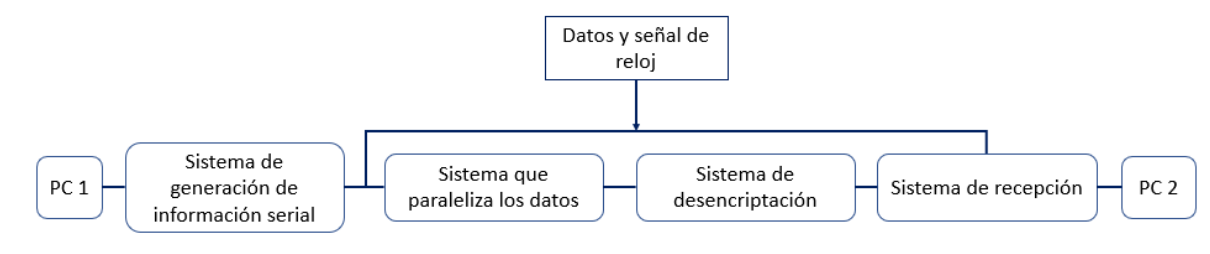
\includegraphics[width=12cm]{imagen/Sistema.png}
    \centering
    \caption{Esquema del sistema}
    \label{fig:Sistema}
    \end{figure}

\section{75HC595}
\subsection{Un breve vistazo}
El 75HC595 es un circuito integrado digital, recibe los datos de entrada en forma serial,  hasta ocho bits, y entrega sus datos a la salida de forma paralela. 

El circuito integrado 75HC595 tiene un empaquetado de 16 puertos, donde el norte se caracteriza por una entrada de medio óvalo. Los datos los recibe por el pin SER  y la salida de datos en paralelo se da por los pines Qa al Qh. Se tiene también un pin de tierra GND, un pin de energía VCC, un pin Qh' utilizado generalmente para cuando se desean conectar varios de estos integrados en cascadas donde el Qh' salida de un integrado sería la entrada de otro integrado. También se encuentran los pines SRCLK (reloj de registro de desplazamiento) y RCLK (reloj de registro de almacenamiento) correspondientes a la primer y segunda etapa respectivamente. Por último están los pines $\overline{SRCLR}$ y $\overline{OE}$, donde $\overline{OE}$ es el encargado de habilitar o desabilitar los pines de salida mientras que $\overline{SRCLR}$ puede borrar o no los datos del circuito integrado, dependiendo de si su estado es LOW o HIGH. 

    \begin{figure}[h]
    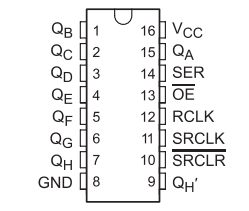
\includegraphics[width=6cm]{imagen/Pines ci.png}
    \centering
    \caption{Vista superior 75HC595}
    \label{fig:Pines ci}
    \end{figure}

\newpage
\subsection{Explicación de la esctructura Interna}

En la figura 3 se puede ver la esctructura interna del 75HC595, esta estructura es del proveedor Texas Instruments \cite{Datasheet}, se divide en dos etapas, la etapa uno se encarga del desplazamiento de del bit que entra, estos flipflop se encuentran conectados en cascada para el desplazamiento del bit, la segunda estapa se encarga de almacenar los bit para cuando se de la orden de salida


\begin{figure}[H]
    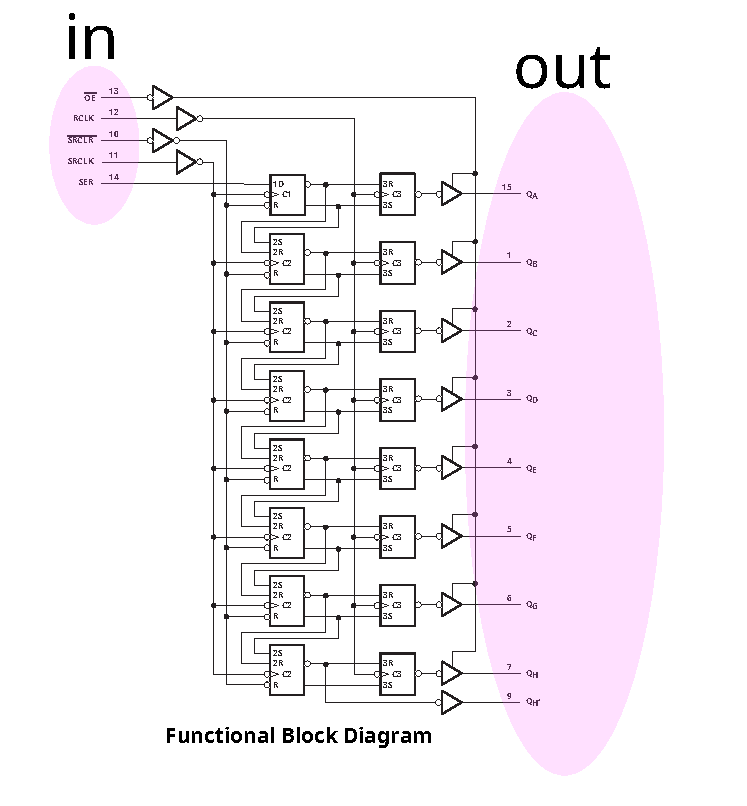
\includegraphics[width=8cm,angle=0, height=10cm ]{imagen/estructuraInterna.pdf}
    \centering
    \caption{Estructura Interna}
    \label{fig:Estructura Interna}
    \end{figure}

\subsection{Como conectar el 75HC595}
En la hoja de datos del circuito integrado se encuentra toda la información referente a la forma de realizar las conexiones de los pines.
    \begin{figure}[h]
    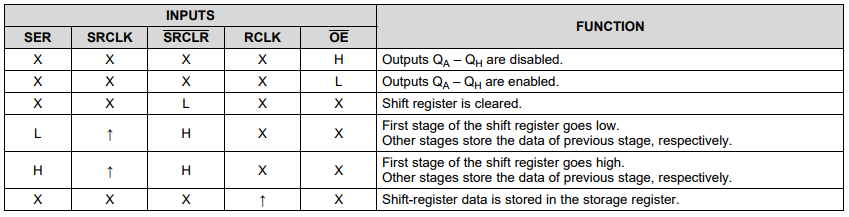
\includegraphics[width=12cm]{imagen/Conexiones.png}
    \centering
    \caption{Modos funcionales 75HC595}
    \label{fig:diagrama}
    \end{figure}
    
Los pines Qa al Qh son los pines de salida donde se obtendran los datos de forma paralela. El pin GND se conecta a la tierra del sistema. El pin VCC es la energía del dispositivo, para este proyecto en particular se conecta al puerto que entrega 5v de la placa arduino. Al pin SER se conectan los datos de entrada, los cuales ingresan en forma serial. El pin $\overline{OE}$ se conecta a tierra para que quede en estado \textit{LOW}, pues estando en \textit{LOW} activa las salidas lo cual es precisamente lo que necesitamos. $\overline{SRCLR}$ se conecta a \textit{VCC} para desactivarlo, pues de tenerlo activado borraría el registro. Por su parte los pines RCKL y SRCLK se conectan cada uno a un pin de salida de la



\subsection{Aplicaciones y algunos ejemplos}
Entre sus aplicaciones se encuentran usos p ara s


\section{Explicación de la arquitectura} 

\section{Explicación del código} 

\subsection{Esquema donde describa las tareas que usted definió en el desarrollo del algoritmo}


\subsection{Algoritmo implementado}
Se parte de que el usuario es el que ingresa los datos por el monitor serial
El grupo decidio partir de los conocimientos de arduino para empezar el montaje de la protoboard en la pagina de simulacion Tinkercad, segun las instruciones del parcial, realizar una matriz de leds 8x8.
Quedaran organizados los leds de la siguiente forma.
    
    \begin{figure}[h]
    \includegraphics[width=6cm]{diagrama.png}
    \centering
    \caption{diagrama de flujo}
    \label{fig:diagrama}
    \end{figure}

\subsection{Problemas de desarrollo que presentó}
De los problemas que surgieron en el desarrolo se destaca el tiempo, pues implico dedicarle mucho tiempo ya que habian otras materias que requerian dicho tiempo, ademas trabajar a distancia con los compañeros no siempre fue acorde a los horarios de cada uno, hay que añadir que el grupo se tuvo que familiarizar con la plataforma y el funcionamiento del integrado.
La parte mas complicada de implementar fue usar los punteros, arreglos y la mamemoria dinamica para ingresar y reproducir los patrones continuamente en la matriz de leds.

\section{Evolución del algoritmo y consideraciones a tener en cuenta en la implementación} 
\label{contenido}
\subsection{Evolucion}
En el desarrolo del algoritmo el principal problema fue entender el funcionamiento de la matriz de leds formada por los circuitos integrados, el cual se definio en un funcionamiento lineal de filas con posiciones encendidas y apagadas, la clave fue tomar en cuenta la sincronia de los relojes de desplazamiento y de salida para encender fila por fila en la matriz;para ingresar un patron en la matriz nos valimos que funcione de tal forma; que por medio de los relojes fuera recorriendo uno por uno los leds de la matriz e ir desplazando un "1" o un "0" para ir dando forma al patron.

\subsection{Resistencias}
En esta seccion se conectan los leds a resistencias.
    \begin{figure}[h]
    \centering
    \includegraphics[width=6cm]{image1.jpg}
    \caption{Union de resistencias}
    \label{fig:image1}
    \end{figure}

\subsection{Circuito Integrado}
Luego de unir las resistencias correspondientes a cada uno de los leds, se conectan las salidas de los 8 ciruitos integrados 74HC595 que se implementaran para ampliar la cantidad de salidas digitales con sus respectivas tierras y activaciones de salida .
    \begin{figure}[h]
    \includegraphics[width=6cm]{image2.jpg}
    \centering
    \caption{Union a 74HC595}
    \label{fig:image2}
    \end{figure}

\subsection{Potencias}
Aqui integramos la potencia de voltaje del arduino a los circuitos integrados, uniendolos en cadena al igual que las entradas de los circuitos integrados asignadas a borrar el registro de desplazamiento.
    \begin{figure}[h]
    \includegraphics[width=6cm]{image3.jpg}
    \centering
    \caption{Potencias}
    \label{fig:image3}
    \end{figure}

\subsection{Entradas}
Se conectan las entradas, reloj de registro de desplazmiento, reloj de registro de salida y las entradas con las las salidas invertidas quedaron ecadenadas entre los 8 circuitos integrados.\cite{datasheet}
    \begin{figure}[h]
    \includegraphics[width=6cm]{image4.png}
    \centering
    \caption{Entradas y salidas}
    \label{fig:image4}
    \end{figure}

\section{Codigo} 
\label{Elaboracion}
\subsection{Inicio}
Se definen las variables para las entradas y salidas seriales.
    \begin{figure}[h]
    \includegraphics[width=7cm]{variables1.png}
    \centering
    \caption{Puertos seriales definidos}
    \label{fig:variables1}
    \end{figure}

\subsection{Prueba}
Se verifica el encedido de todos los leds, se usa la declaracion "int8 t" en el codigo original para reducir memoria de almacenamiento y mejorar el funcionamiento del codigo.
    \begin{figure}[h]
    \includegraphics[width=7cm]{prueba.png}
    \centering
    \caption{Prueba leds}
    \label{fig:prueba}
    \end{figure}

\subsection{Menu}
Se crea un menu en el cual se definen tres opciones de uso.
    \begin{figure}[h]
    \includegraphics[width=7cm]{menu.png}
    \centering
    \caption{menu}
    \label{fig:menu}
    \end{figure}

\subsection{Funcion Publik()}
Para el desarrollo de esta funcion se hizo uso de arreglos, punteros y memoria dinamica. La matriz se crea de forma dinamica ya que su tamaño depende de el numero de patrones que el usuario desee ver puesto que en la solucion que se planteo, decidimos guardar todos los patrones en una misma matriz; a la misma vez que el usuario ingrese todos los patrones se guardan en la matriz, apenas se llene la matriz se procede a enviar los datos alojados en la matriz al pin de entrada de datos del circuito integrado.
Para visualizar un patron aparte del otro se añade un delay cada 8 filas lo que corresponde a cada patron diferente,para esto se implemento el contador NumFila, este es el encargado de mostrar cuando se completo un patron.

\begin{figure}
 \centering
  \subfloat[Publik1]{
   \label{f:publik1}
    \includegraphics[width=0.2\textwidth]{publik1.jpeg}}
  \subfloat[Publik2]{
   \label{f:publik2}
    \includegraphics[width=0.3\textwidth]{publik2.jpeg}}
  \subfloat[Publik3]{
   \label{f:Publik3}
    \includegraphics[width=0.2\textwidth]{publik3.jpeg}}
   \subfloat[Publik4]{
    \label{f:Publik4}
     \includegraphics[width=0.2\textwidth]{publik4.jpeg}}
   \subfloat[Publik5]{
    \label{f:Publik5}
     \includegraphics[width=0.2\textwidth]{publik5.jpeg}}
 \caption{Funcion Publik}
 \label{f:Publik}
\end{figure}
    

\subsection{Opciones}
Se usa la funcion switch para ingresar a la opcion deseada y en cada case, se define el funcionamiento de las opciones a elegir.
    \begin{figure}[h]
    \includegraphics[width=6cm]{opciones.png}
    \centering
    \caption{Opciones de uso en Switch}
    \label{fig:opciones}
    \end{figure}


\section{Conclusiones} 
\label{Algoritmo}



\bibliographystyle{IEEEtran}
\bibliography{references}

\end{document}